\documentclass[12pt]{article}

% ============================================================
% Packages
% ============================================================
\usepackage[a4paper, margin=2.5cm]{geometry}
\usepackage{amsmath, amssymb, amsfonts}
\usepackage{graphicx}
\usepackage{booktabs}
\usepackage{hyperref}
\usepackage{cleveref}
\usepackage{float}
\usepackage{subcaption}
\usepackage{algorithm}
\usepackage{algpseudocode}
\usepackage{bm}
\usepackage{natbib}
\usepackage{xcolor}
\usepackage{tikz}
\usepackage{pgfplots}
\usepackage{multirow}
\usepackage{enumitem}
\usepackage{tabularx}

\usetikzlibrary{arrows.meta, positioning, shapes.geometric, fit, calc, backgrounds, decorations.markings, patterns}
\pgfplotsset{compat=1.18}

\hypersetup{
    colorlinks=true,
    linkcolor=blue,
    citecolor=blue,
    urlcolor=blue
}

% ============================================================
% Custom commands
% ============================================================
\newcommand{\R}{\mathbb{R}}
\newcommand{\norm}[1]{\left\| #1 \right\|}
\newcommand{\abs}[1]{\left| #1 \right|}
\newcommand{\tensor}[1]{\boldsymbol{\mathcal{#1}}}
\newcommand{\mat}[1]{\mathbf{#1}}
\newcommand{\vect}[1]{\mathbf{#1}}
\newcommand{\dt}{\Delta t}

% Colour palette for TikZ
\definecolor{agentblue}{RGB}{52, 119, 198}
\definecolor{agentgreen}{RGB}{46, 139, 87}
\definecolor{agentorange}{RGB}{230, 126, 34}
\definecolor{agentred}{RGB}{192, 57, 43}
\definecolor{agentpurple}{RGB}{142, 68, 173}
\definecolor{agentgray}{RGB}{127, 140, 141}
\definecolor{llmgold}{RGB}{241, 196, 15}
\definecolor{reviewerpink}{RGB}{231, 76, 60}
\definecolor{lightbg}{RGB}{245, 248, 252}

\graphicspath{{figures/}}

% ============================================================
\title{A Multi-Agent AI Framework Integrating Large Language Models and Machine Learning for Wind Turbine Predictive Maintenance and Wake Steering Optimisation}

\author{
  Mandar Tabib \\
  \textit{SINTEF Digital, Department of Mathematics and Cybernetics} \\
  \textit{Trondheim, Norway} \\
  mandar.tabib@sintef.no
}

\date{}

% ============================================================
\begin{document}
\maketitle

% ============================================================
% ABSTRACT
% ============================================================
\begin{abstract}
This report presents a multi-agent artificial intelligence framework---\textsc{AeroAgent}---that orchestrates Large Language Models (LLMs) alongside domain-specific machine learning surrogates for real-time wind turbine operational analysis, wake steering optimisation, and predictive maintenance.
The system comprises six specialised agents: (1)~a weather data acquisition agent interfacing with meteorological APIs, (2)~a dual rule-based and LLM-powered turbine expert for yaw and pitch recommendations, (3)~a wake steering optimiser for multi-turbine farm-level power maximisation, (4)~a Tensor Train--Operator Inference (TT-OpInf) reduced-order model for three-dimensional wake velocity field prediction, (5)~a Gaussian Process Regression (GPR) surrogate for uncertainty-aware rotor power prediction, and (6)~a predictive maintenance module combining autoencoders, Gaussian Mixture Models, and gradient boosting classifiers for health state estimation and Remaining Useful Life (RUL) prediction.
An asynchronous expert reviewer agent, itself LLM-powered, validates outputs at critical checkpoints in either advisory or blocking mode.
The framework supports five interchangeable LLM providers through a factory abstraction pattern and is deployed via a Streamlit web interface with integrated three-dimensional visualisation.
SHAP-based explainability is embedded throughout to ensure transparency of model predictions.
Performance benchmarks from the constituent models include a $10.1\times$ data compression with 12.9\% relative $L^2$ error for wake flow prediction, RMSE of 0.048~MW ($R^2 = 0.70$) for power prediction, and a weighted F1-score of 0.75 for multi-class fault prediction on real SCADA data from Fuhrlander FL2500 turbines.
\end{abstract}

\noindent\textbf{Keywords:} multi-agent system, large language model, wind turbine, predictive maintenance, wake steering, reduced-order model, Gaussian process, SHAP explainability, SCADA

% ============================================================
% 1. INTRODUCTION
% ============================================================
\section{Introduction}
\label{sec:introduction}

Wind energy has become a cornerstone of the global transition to renewable power, yet two persistent challenges constrain wind farm profitability: wake-induced power losses and unplanned maintenance downtime.
Downstream turbines can experience power deficits of 10--20\% due to reduced wind speed and increased turbulence within upstream wakes \citep{Barthelmie2009, PorteAgel2020}, while maintenance costs account for 20--35\% of the total cost of energy, with gearbox failures alone requiring 5--10 days of downtime per event \citep{tchakoua2014, sheng2013}.

Intentional yaw misalignment---\emph{wake steering}---deflects the wake laterally away from downstream rotors, thereby increasing aggregate farm power output \citep{Fleming2017, Gebraad2016}.
Effective implementation requires fast, accurate predictions of both the three-dimensional wake velocity field and the corresponding rotor power under varying yaw angles.
Simultaneously, condition-based maintenance scheduling demands real-time health monitoring from Supervisory Control and Data Acquisition (SCADA) data streams that capture thermal, mechanical, and electrical signatures of normal operation and degradation.

Recent advances in Large Language Models (LLMs) have demonstrated remarkable capabilities in reasoning, domain-specific question answering, and structured output generation \citep{Brown2020}.
Concurrently, multi-agent systems (MAS) have a long history in distributed artificial intelligence, where autonomous agents with specialised capabilities cooperate to solve complex problems that exceed the capacity of any single agent \citep{Wooldridge2009, Dorri2018}.
The emergence of LLM-based autonomous agents \citep{Xi2023, Wang2024} presents an opportunity to combine the reasoning capabilities of language models with the computational precision of domain-specific machine learning surrogates.

This work presents \textsc{AeroAgent}, a multi-agent AI framework that integrates LLMs as expert reasoners and reviewers with physics-informed machine learning models for wind turbine operations.
The principal contributions are:

\begin{enumerate}[leftmargin=*]
    \item A \textbf{multi-agent orchestration architecture} comprising six specialised agents and an LLM-powered expert reviewer, coordinated through an asynchronous checkpoint-based pipeline.
    \item Integration of \textbf{three domain-specific ML surrogates}: TT-OpInf for wake flow prediction \citep{Tabib2025ttopinf}, GPR for power prediction with uncertainty quantification \citep{Tabib2025gpr}, and a semi-supervised autoencoder--GMM--classifier pipeline for predictive maintenance \citep{Tabib2025pdm}.
    \item A \textbf{multi-provider LLM abstraction layer} supporting five providers (NTNU HPC, OpenAI, Anthropic, Google, Ollama) through a unified asynchronous interface with a factory design pattern.
    \item \textbf{SHAP-based model explainability} embedded at each prediction stage to ensure transparency and build operator trust.
    \item A \textbf{deployable web application} with real-time weather integration, three-dimensional wake visualisation, and Norwegian wind farm support.
\end{enumerate}

The remainder of this report is organised as follows.
\Cref{sec:architecture} describes the multi-agent system architecture and orchestration protocol.
\Cref{sec:ml_methods} summarises the constituent machine learning methods.
\Cref{sec:llm_integration} details the LLM integration and expert reviewer system.
\Cref{sec:optimisation} presents the wake steering optimisation framework.
\Cref{sec:implementation} discusses the software implementation.
\Cref{sec:results} presents results and discussion, and \Cref{sec:conclusion} concludes with directions for future work.


% ============================================================
% 2. SYSTEM ARCHITECTURE
% ============================================================
\section{Multi-Agent System Architecture}
\label{sec:architecture}

\subsection{Overview}
\label{sec:arch_overview}

The \textsc{AeroAgent} framework follows a cooperative multi-agent paradigm \citep{Dorri2018} in which specialised agents communicate through a centralised orchestrator.
Each agent encapsulates a distinct operational capability---data acquisition, expert reasoning, surrogate model inference, or health monitoring---and exposes a standardised interface for input consumption and output production.
The orchestrator manages agent sequencing, data routing, and invocation of the expert reviewer at predefined checkpoints.

\Cref{fig:architecture} provides a high-level view of the multi-agent architecture.
The six primary agents are colour-coded by functional category: data acquisition (blue), expert analysis (green), machine learning prediction (orange), and health monitoring (red).

% ============================================================
% FIGURE 1: Multi-Agent Architecture Overview
% ============================================================
\begin{figure}[H]
\centering
\resizebox{\textwidth}{!}{%
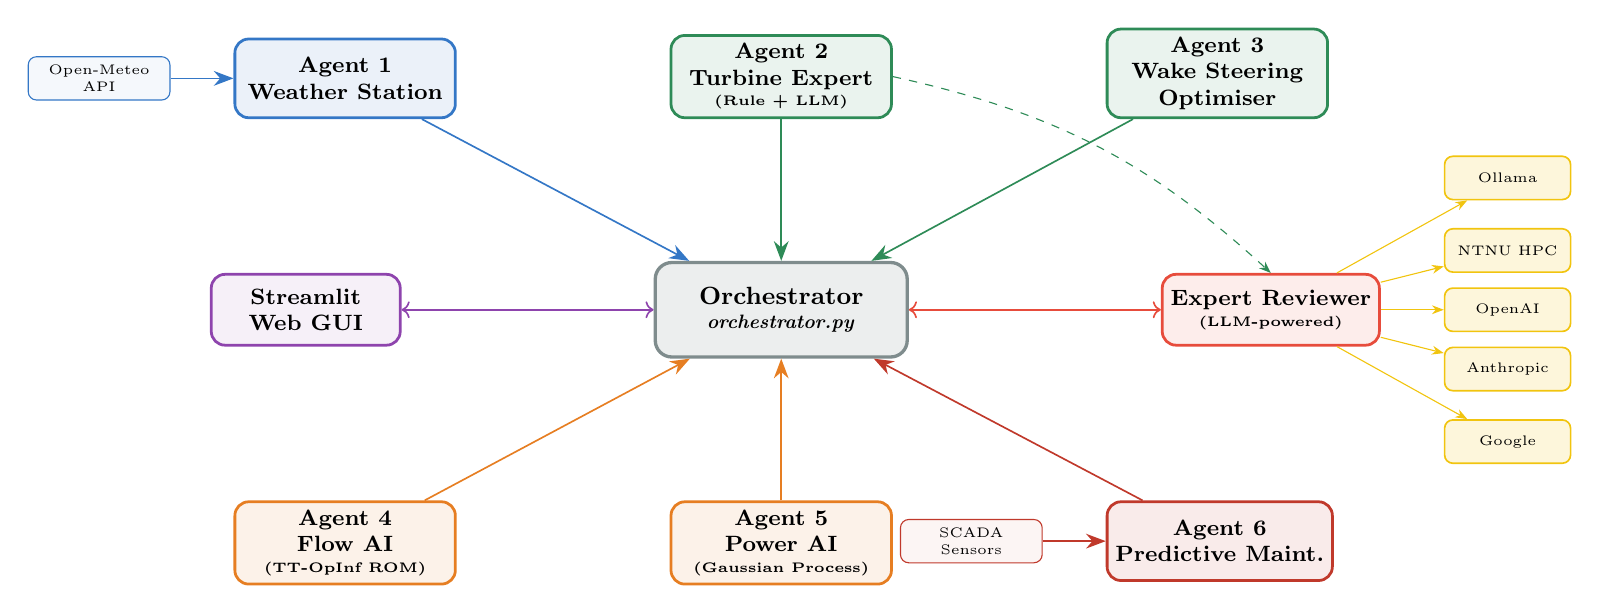
\begin{tikzpicture}[
    agent/.style={rectangle, rounded corners=5pt, draw=#1, fill=#1!10, line width=1pt, minimum width=2.8cm, minimum height=1.0cm, align=center, font=\footnotesize\bfseries},
    orchestrator/.style={rectangle, rounded corners=6pt, draw=agentgray, fill=agentgray!15, line width=1.2pt, minimum width=3.2cm, minimum height=1.2cm, align=center, font=\small\bfseries},
    reviewer/.style={rectangle, rounded corners=5pt, draw=reviewerpink, fill=reviewerpink!10, line width=1pt, minimum width=2.6cm, minimum height=0.9cm, align=center, font=\footnotesize\bfseries},
    llmprov/.style={rectangle, rounded corners=3pt, draw=llmgold, fill=llmgold!15, line width=0.6pt, minimum width=1.6cm, minimum height=0.55cm, align=center, font=\tiny},
    dataflow/.style={-{Stealth[length=2.5mm]}, semithick, color=#1},
    every node/.style={inner sep=3pt}
]

% Orchestrator (centre)
\node[orchestrator] (orch) at (0,0) {Orchestrator\\[-2pt]\scriptsize\textit{orchestrator.py}};

% Agent 1: Weather (top-left)
\node[agent=agentblue, above left=1.8cm and 2.5cm of orch] (a1) {Agent 1\\Weather Station};

% Agent 2: Expert (top)
\node[agent=agentgreen, above=1.8cm of orch] (a2) {Agent 2\\Turbine Expert\\[-2pt]\tiny (Rule + LLM)};

% Agent 3: Optimizer (top-right)
\node[agent=agentgreen, above right=1.8cm and 2.5cm of orch] (a3) {Agent 3\\Wake Steering\\Optimiser};

% Agent 4: Wake Flow (bottom-left)
\node[agent=agentorange, below left=1.8cm and 2.5cm of orch] (a4) {Agent 4\\Flow AI\\[-2pt]\tiny (TT-OpInf ROM)};

% Agent 5: Power (bottom)
\node[agent=agentorange, below=1.8cm of orch] (a5) {Agent 5\\Power AI\\[-2pt]\tiny (Gaussian Process)};

% Agent 6: PdM (bottom-right)
\node[agent=agentred, below right=1.8cm and 2.5cm of orch] (a6) {Agent 6\\Predictive Maint.};

% Expert Reviewer (right)
\node[reviewer, right=3.2cm of orch] (rev) {Expert Reviewer\\[-2pt]\tiny (LLM-powered)};

% LLM Providers (stacked to the right of reviewer)
\node[llmprov, above right=0.0cm and 0.8cm of rev] (llm1) {NTNU HPC};
\node[llmprov, right=0.8cm of rev] (llm2) {OpenAI};
\node[llmprov, below right=0.0cm and 0.8cm of rev] (llm3) {Anthropic};
\node[llmprov, below=0.35cm of llm3] (llm4) {Google};
\node[llmprov, above=0.35cm of llm1] (llm5) {Ollama};

% External data (left)
\node[rectangle, rounded corners=3pt, draw=agentblue, fill=agentblue!5, minimum width=1.8cm, minimum height=0.55cm, font=\tiny, align=center, left=0.8cm of a1] (weather) {Open-Meteo\\API};

\node[rectangle, rounded corners=3pt, draw=agentred, fill=agentred!5, minimum width=1.8cm, minimum height=0.55cm, font=\tiny, align=center, left=0.8cm of a6] (scada) {SCADA\\Sensors};

% GUI (left of orchestrator)
\node[rectangle, rounded corners=5pt, draw=agentpurple, fill=agentpurple!8, line width=1pt, minimum width=2.4cm, minimum height=0.9cm, font=\footnotesize\bfseries, align=center, left=3.2cm of orch] (gui) {Streamlit\\Web GUI};

% Arrows: Agents to Orchestrator
\draw[dataflow=agentblue] (a1) -- (orch);
\draw[dataflow=agentgreen] (a2) -- (orch);
\draw[dataflow=agentgreen] (a3) -- (orch);
\draw[dataflow=agentorange] (a4) -- (orch);
\draw[dataflow=agentorange] (a5) -- (orch);
\draw[dataflow=agentred] (a6) -- (orch);

% Arrows: Orchestrator to Reviewer
\draw[dataflow=reviewerpink, <->] (orch) -- (rev);

% Arrows: Reviewer to LLM providers
\draw[-{Stealth[length=1.5mm]}, thin, color=llmgold] (rev) -- (llm1);
\draw[-{Stealth[length=1.5mm]}, thin, color=llmgold] (rev) -- (llm2);
\draw[-{Stealth[length=1.5mm]}, thin, color=llmgold] (rev) -- (llm3);
\draw[-{Stealth[length=1.5mm]}, thin, color=llmgold] (rev) -- (llm4);
\draw[-{Stealth[length=1.5mm]}, thin, color=llmgold] (rev) -- (llm5);

% External data arrows
\draw[dataflow=agentblue] (weather) -- (a1);
\draw[dataflow=agentred] (scada) -- (a6);

% GUI arrow
\draw[dataflow=agentpurple, <->] (gui) -- (orch);

% Agent 2 to LLM (via reviewer path)
\draw[-{Stealth[length=1.5mm]}, dashed, thin, color=agentgreen] (a2.east) to[bend left=15] (rev.north);

\end{tikzpicture}%
}% end resizebox
\caption{High-level multi-agent architecture of the \textsc{AeroAgent} framework. Six specialised agents (colour-coded by function) communicate through a centralised orchestrator. An LLM-powered expert reviewer validates outputs at critical checkpoints. Five interchangeable LLM providers are accessible through a unified factory interface.}
\label{fig:architecture}
\end{figure}


\subsection{Agent Descriptions}
\label{sec:agent_descriptions}

\Cref{tab:agents} summarises the six primary agents and the expert reviewer.

\begin{table}[H]
\centering
\caption{Summary of agents in the \textsc{AeroAgent} framework.}
\label{tab:agents}
\small
\begin{tabularx}{\textwidth}{c l l X}
\toprule
\textbf{ID} & \textbf{Agent} & \textbf{Type} & \textbf{Description} \\
\midrule
1 & Weather Station & Data acquisition & Fetches real-time wind speed, direction, and temperature from the Open-Meteo API for a specified location. \\
2 & Turbine Expert & Rule-based + LLM & Dual-mode expert: (2A) deterministic NREL 5\,MW reference turbine specifications with operating region classification; (2B) LLM-based yaw and pitch recommendation. \\
3 & Wake Steering Optimiser & Optimisation & Multi-turbine farm-level yaw optimisation for aggregate power maximisation using wake deficit models. \\
4 & Flow AI & ML surrogate & TT-OpInf reduced-order model predicting three-component velocity fields ($u_x, u_y, u_z$) on 180{,}857 spatial nodes under varying yaw angles. \\
5 & Power AI & ML surrogate & Gaussian Process Regression model predicting transient rotor power with uncertainty quantification (95\% confidence intervals). \\
6 & Predictive Maintenance & ML pipeline & Four-stage semi-supervised framework: autoencoder $\to$ GMM $\to$ supervised classifier $\to$ RUL estimation. \\
\midrule
R & Expert Reviewer & LLM-powered & Asynchronous validation at three checkpoints (post-Agent~2, post-Agent~5, post-Agent~4) in advisory or blocking mode. \\
\bottomrule
\end{tabularx}
\end{table}


\subsection{Orchestration Protocol}
\label{sec:orchestration}

The orchestrator implements a sequential pipeline with asynchronous reviewer checkpoints.
\Cref{fig:pipeline} illustrates the execution flow.

% ============================================================
% FIGURE 2: Orchestration Pipeline
% ============================================================
\begin{figure}[H]
\centering
\resizebox{\textwidth}{!}{%
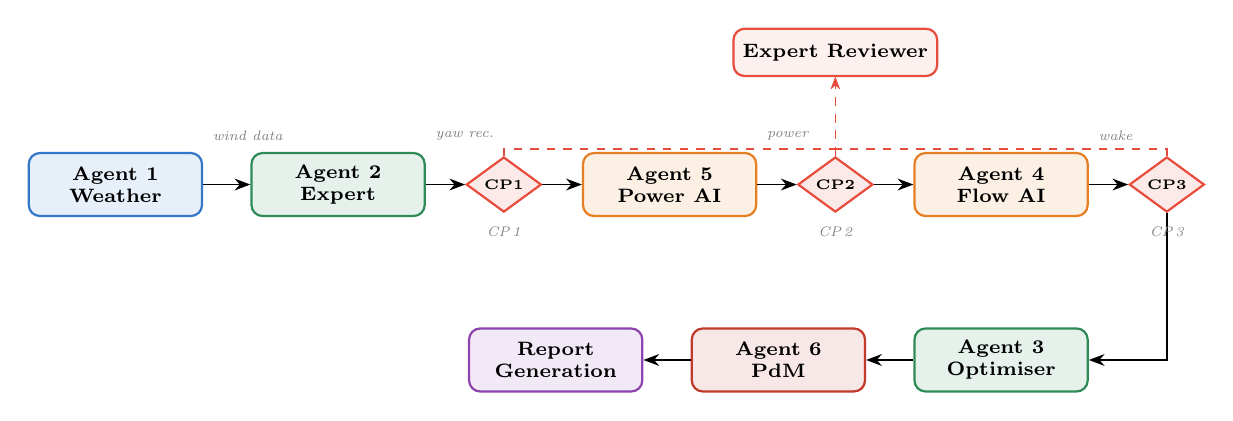
\begin{tikzpicture}[
    step/.style={rectangle, rounded corners=4pt, draw=#1, fill=#1!12, line width=0.8pt, minimum width=2.2cm, minimum height=0.8cm, align=center, font=\scriptsize\bfseries},
    checkpoint/.style={diamond, draw=reviewerpink, fill=reviewerpink!12, line width=0.8pt, minimum width=0.8cm, minimum height=0.7cm, align=center, font=\tiny\bfseries, inner sep=1pt, aspect=2},
    arr/.style={-{Stealth[length=2mm]}, semithick},
    darr/.style={-{Stealth[length=1.5mm]}, semithick, dashed, color=reviewerpink},
    note/.style={font=\tiny\itshape, color=gray}
]

% Row 1: Pipeline nodes
\node[step=agentblue] (s1) at (0,0) {Agent 1\\Weather};
\node[step=agentgreen, right=0.6cm of s1] (s2) {Agent 2\\Expert};
\node[checkpoint, right=0.5cm of s2] (c1) {CP1};
\node[step=agentorange, right=0.5cm of c1] (s5) {Agent 5\\Power AI};
\node[checkpoint, right=0.5cm of s5] (c2) {CP2};
\node[step=agentorange, right=0.5cm of c2] (s4) {Agent 4\\Flow AI};
\node[checkpoint, right=0.5cm of s4] (c3) {CP3};

% Row 2
\node[step=agentgreen, below=1.4cm of s4] (s3) {Agent 3\\Optimiser};
\node[step=agentred, left=0.6cm of s3] (s6) {Agent 6\\PdM};
\node[step=agentpurple, left=0.6cm of s6] (report) {Report\\Generation};

% Arrows
\draw[arr] (s1) -- (s2);
\draw[arr] (s2) -- (c1);
\draw[arr] (c1) -- (s5);
\draw[arr] (s5) -- (c2);
\draw[arr] (c2) -- (s4);
\draw[arr] (s4) -- (c3);
\draw[arr] (c3) |- (s3);
\draw[arr] (s3) -- (s6);
\draw[arr] (s6) -- (report);

% Reviewer node
\node[rectangle, rounded corners=4pt, draw=reviewerpink, fill=reviewerpink!8, line width=0.8pt, minimum width=2.0cm, minimum height=0.6cm, align=center, font=\scriptsize\bfseries, above=1.0cm of c2] (rev) {Expert Reviewer};

% Reviewer connections
\draw[darr] (c1) -- ++(0,0.45) -| (rev);
\draw[darr] (c2) -- (rev);
\draw[darr] (c3) -- ++(0,0.45) -| (rev);

% Labels
\node[note, below=0.05cm of c1] {CP\,1};
\node[note, below=0.05cm of c2] {CP\,2};
\node[note, below=0.05cm of c3] {CP\,3};

% Data flow annotations
\node[note, above=0.02cm of s1.north east, anchor=south west] {wind data};
\node[note, above=0.02cm of s2.north east, anchor=south west] {yaw rec.};
\node[note, above=0.02cm of s5.north east, anchor=south west] {power};
\node[note, above=0.02cm of s4.north east, anchor=south west] {wake};

\end{tikzpicture}%
}% end resizebox
\caption{Agent orchestration pipeline with reviewer checkpoints (CP1--CP3). Dashed arrows indicate asynchronous LLM-based validation. In advisory mode, the reviewer provides feedback without blocking; in blocking mode, critical issues halt the pipeline.}
\label{fig:pipeline}
\end{figure}

The orchestrator proceeds as follows:
\begin{enumerate}[leftmargin=*]
    \item \textbf{Agent~1} (Weather Station) fetches real-time meteorological conditions---wind speed $v_\infty$ (m/s), wind direction $\theta_w$ (degrees), and ambient temperature $T_a$ ($^\circ$C)---from the Open-Meteo API for a user-specified geographic location.
    \item \textbf{Agent~2} (Turbine Expert) receives the weather data and produces yaw and pitch recommendations. Agent~2A applies deterministic rules based on the NREL 5\,MW reference turbine operating regions (below cut-in at $v < 3$\,m/s, Region~2 partial load, Region~3 full load, above cut-out at $v > 25$\,m/s). Agent~2B queries an LLM for a complementary recommendation.
    \item \textbf{Checkpoint~1}: The expert reviewer validates the yaw recommendation against physical constraints (yaw range, operating region consistency, wind speed limits).
    \item \textbf{Agent~5} (Power AI) predicts rotor power as a function of the recommended yaw angle using a pre-trained Gaussian Process model, returning mean predictions with 95\% confidence intervals.
    \item \textbf{Checkpoint~2}: The reviewer validates power predictions (range plausibility, uncertainty bounds).
    \item \textbf{Agent~4} (Flow AI) predicts the three-dimensional wake velocity field using the TT-OpInf ROM, optionally exporting VTK files for visualisation.
    \item \textbf{Checkpoint~3}: The reviewer validates wake predictions (velocity magnitude range, spatial consistency).
    \item \textbf{Agent~3} (Wake Steering Optimiser) and \textbf{Agent~6} (Predictive Maintenance) execute in parallel, using outputs from previous agents.
    \item A comprehensive report is generated aggregating all agent outputs.
\end{enumerate}

The reviewer operates in two configurable modes:
\begin{itemize}[leftmargin=*]
    \item \textbf{Advisory mode}: Feedback is appended to the report but never blocks the pipeline. This is the default for exploratory analyses.
    \item \textbf{Blocking mode}: Critical issues (e.g., yaw angle outside physical limits, power exceeding rated capacity) halt execution until resolved.
\end{itemize}

Each reviewer checkpoint first applies deterministic rule-based checks (boundary validation, consistency checks) before optionally invoking the LLM for higher-level reasoning about the plausibility of results.


% ============================================================
% 3. MACHINE LEARNING METHODS
% ============================================================
\section{Machine Learning Methods}
\label{sec:ml_methods}

This section summarises the three domain-specific ML methods integrated as agents.
Detailed derivations and standalone evaluations are presented in companion papers \citep{Tabib2025ttopinf, Tabib2025gpr, Tabib2025pdm}.

\subsection{Wake Flow Prediction via TT-OpInf (Agent~4)}
\label{sec:ttopinf}

Agent~4 employs the Tensor Train--Operator Inference (TT-OpInf) reduced-order model to predict three-component velocity fields ($u_x, u_y, u_z$) at 180{,}857 unstructured mesh nodes under varying yaw angles.

\subsubsection{Tensor Train Decomposition}

Given a four-dimensional data tensor $\tensor{X} \in \R^{N_\mu \times N_t \times N_s \times N_f}$ (parameter $\times$ time $\times$ space $\times$ feature), the TT decomposition \citep{Oseledets2011} factorises $\tensor{X}$ into a chain of low-rank cores:
\begin{equation}
    \tensor{X}(\mu, t, s, f) \approx \mat{G}_1(\mu, :) \cdot \mat{G}_2(:, t, :) \cdot \mat{G}_3(:, sf)
    \label{eq:tt_decomp}
\end{equation}
where $\mat{G}_1 \in \R^{N_\mu \times r_1}$ is the parameter core, $\mat{G}_2 \in \R^{r_1 \times N_t \times r_2}$ is the temporal core, and $\mat{G}_3 \in \R^{r_2 \times (N_s \cdot N_f)}$ is the spatial core.
The TT-ranks $(r_1, r_2)$ are determined by an energy-based truncation criterion applied to the singular value decomposition (SVD) at each unfolding.

\subsubsection{Operator Inference}

Following \citet{Peherstorfer2016}, a linear dynamical system is learned from the temporal coefficients extracted from $\mat{G}_2$:
\begin{equation}
    \frac{d\vect{g}}{dt} = \vect{c} + \mat{A}_1 \vect{g}
    \label{eq:opinf}
\end{equation}
where $\vect{g}(t) \in \R^{r_2}$ are the time coefficients for a given parameter value, $\vect{c}$ is a constant vector, and $\mat{A}_1$ is the state matrix.
The operators $(\vect{c}, \mat{A}_1)$ are obtained via Tikhonov-regularised least squares:
\begin{equation}
    \min_{\vect{c}, \mat{A}_1} \norm{\dot{\mat{G}} - [\mathbf{1} \mid \mat{G}] \begin{bmatrix} \vect{c}^T \\ \mat{A}_1^T \end{bmatrix}}_F^2 + \lambda \norm{\begin{bmatrix} \vect{c}^T \\ \mat{A}_1^T \end{bmatrix}}_F^2
\end{equation}
Temporal integration of \eqref{eq:opinf} is performed using a fourth-order Runge--Kutta (RK4) scheme.

\subsubsection{Parametric Interpolation}

For prediction at unseen yaw angles $\mu^*$, the parameter core $\mat{G}_1$ is interpolated using thin-plate-spline radial basis functions (RBF):
\begin{equation}
    \mat{G}_1(\mu^*) = \sum_{i=1}^{N_\mu} w_i \, \phi(\norm{\mu^* - \mu_i})
\end{equation}
where $\phi(r) = r^2 \ln(r)$ is the thin-plate-spline kernel and $\{w_i\}$ are the interpolation weights.

\subsubsection{Performance}

Trained on OpenFOAM simulations at three yaw angles (270$^\circ$, 282$^\circ$, 285$^\circ$) with 101 time steps, the model achieves:
\begin{itemize}[leftmargin=*]
    \item $10.1\times$ data compression ratio
    \item 2.6\% reconstruction error on training data
    \item 12.9\% relative $L^2$ error on held-out yaw angle (276$^\circ$)
    \item Sub-second inference time (no GPU required)
\end{itemize}


\subsection{Rotor Power Prediction via GPR (Agent~5)}
\label{sec:gpr}

Agent~5 employs Gaussian Process Regression \citep{Rasmussen2006} to predict transient rotor power as a function of yaw angle and normalised time.

\subsubsection{Model Formulation}

A Gaussian process defines a distribution over functions $f: \R^2 \to \R$ such that any finite collection of function values is jointly Gaussian:
\begin{equation}
    f(\vect{x}) \sim \mathcal{GP}\bigl(m(\vect{x}),\; k(\vect{x}, \vect{x}')\bigr)
\end{equation}
where $\vect{x} = [\theta_{\text{yaw}},\; \tau]^T$ with $\theta_{\text{yaw}}$ the yaw angle (270$^\circ$--285$^\circ$) and $\tau \in [0, 1]$ the normalised time.
The covariance kernel is a Mat\'{e}rn~$\nu = 5/2$ kernel combined with a white noise kernel:
\begin{equation}
    k(\vect{x}, \vect{x}') = \sigma_f^2 \left(1 + \frac{\sqrt{5}\, r}{\ell} + \frac{5 r^2}{3 \ell^2}\right) \exp\left(-\frac{\sqrt{5}\, r}{\ell}\right) + \sigma_n^2 \delta(\vect{x}, \vect{x}')
\end{equation}
where $r = \norm{\vect{x} - \vect{x}'}$ and hyperparameters $(\sigma_f, \ell, \sigma_n)$ are optimised by maximising the log marginal likelihood.

\subsubsection{Uncertainty Quantification}

The predictive distribution at a test point $\vect{x}_*$ is:
\begin{equation}
    P(y_* \mid \vect{x}_*, \mathcal{D}) = \mathcal{N}\bigl(\mu_*,\; \sigma_*^2\bigr)
\end{equation}
The 95\% confidence interval is $\mu_* \pm 1.96\,\sigma_*$, providing calibrated uncertainty bounds for decision-making.

\subsubsection{Performance}

Trained on 1{,}598 subsampled data points from CFD simulations at four yaw angles, the model achieves RMSE~$= 0.048$~MW and $R^2 = 0.70$ on a held-out test set of 400 samples.


\subsection{Predictive Maintenance (Agent~6)}
\label{sec:pdm}

Agent~6 implements a four-stage semi-supervised framework for health monitoring, validated on real SCADA data from five Fuhrlander FL2500 (2.5\,MW) turbines over three years (2012--2014) \citep{blanco2020}.
\Cref{fig:pdm_pipeline} illustrates the complete predictive maintenance workflow.

% ============================================================
% FIGURE 5: Predictive Maintenance Pipeline
% ============================================================
\begin{figure}[H]
\centering
\resizebox{\textwidth}{!}{%
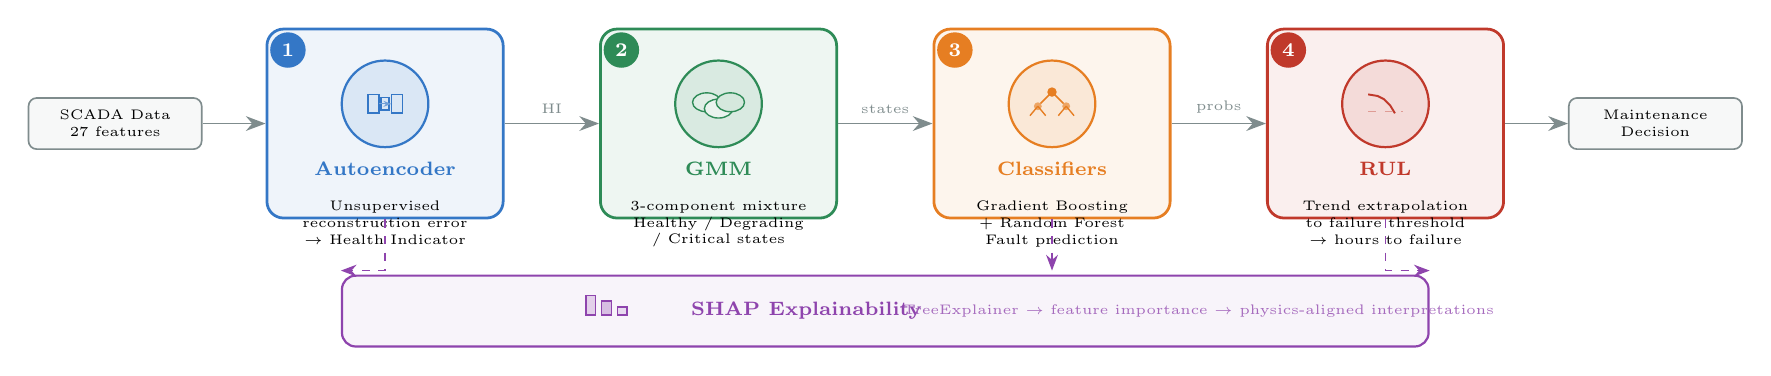
\begin{tikzpicture}[
    stage/.style={rectangle, rounded corners=6pt, draw=#1, fill=#1!8, line width=1pt, minimum width=3.0cm, minimum height=2.4cm, align=center, font=\footnotesize\bfseries},
    icon/.style={circle, draw=#1, fill=#1!18, line width=0.8pt, minimum size=1.1cm, align=center, font=\tiny\bfseries, inner sep=0pt},
    label/.style={font=\tiny, align=center, text width=2.8cm},
    iobox/.style={rectangle, rounded corners=3pt, draw=#1, fill=#1!6, line width=0.6pt, minimum width=2.2cm, minimum height=0.65cm, align=center, font=\tiny},
    arr/.style={-{Stealth[length=2.5mm]}, semithick, color=agentgray},
    dataarr/.style={-{Stealth[length=2mm]}, semithick, color=#1},
    stagenum/.style={circle, fill=#1, text=white, font=\scriptsize\bfseries, minimum size=0.45cm, inner sep=0pt},
]

% ── Stage 1: Autoencoder ──
\node[stage=agentblue] (s1) at (0,0) {};
\node[stagenum=agentblue, anchor=north west] at ([shift={(0.12,-0.12)}]s1.north west) {1};
% AE icon: layered rectangles suggesting encoder-decoder
\node[icon=agentblue] (ae_icon) at ([yshift=0.25cm]s1.center) {};
\draw[agentblue, line width=0.6pt] ([xshift=-0.22cm, yshift=0.12cm]ae_icon.center) rectangle ++(0.14cm,-0.24cm);
\draw[agentblue, line width=0.6pt] ([xshift=-0.05cm, yshift=0.08cm]ae_icon.center) rectangle ++(0.10cm,-0.16cm);
\draw[agentblue, line width=0.6pt] ([xshift=0.08cm, yshift=0.12cm]ae_icon.center) rectangle ++(0.14cm,-0.24cm);
\draw[agentblue!70, line width=0.4pt, -{Stealth[length=1mm]}] ([xshift=-0.08cm]ae_icon.center) -- ++(0.16cm,0);
\node[font=\scriptsize\bfseries, agentblue, below=0.05cm of ae_icon] {Autoencoder};
\node[label, below=0.55cm of ae_icon] {Unsupervised\\reconstruction error\\$\to$ Health Indicator};

% ── Stage 2: GMM ──
\node[stage=agentgreen, right=1.2cm of s1] (s2) {};
\node[stagenum=agentgreen, anchor=north west] at ([shift={(0.12,-0.12)}]s2.north west) {2};
% GMM icon: three overlapping ellipses
\node[icon=agentgreen] (gmm_icon) at ([yshift=0.25cm]s2.center) {};
\draw[agentgreen, line width=0.5pt, fill=agentgreen!15] ([xshift=-0.15cm, yshift=0.02cm]gmm_icon.center) ellipse (0.18cm and 0.12cm);
\draw[agentgreen, line width=0.5pt, fill=agentgreen!10] ([xshift=0.0cm, yshift=-0.06cm]gmm_icon.center) ellipse (0.18cm and 0.12cm);
\draw[agentgreen, line width=0.5pt, fill=agentgreen!20] ([xshift=0.15cm, yshift=0.02cm]gmm_icon.center) ellipse (0.18cm and 0.12cm);
\node[font=\scriptsize\bfseries, agentgreen, below=0.05cm of gmm_icon] {GMM};
\node[label, below=0.55cm of gmm_icon] {3-component mixture\\Healthy / Degrading\\/ Critical states};

% ── Stage 3: Supervised Classifiers ──
\node[stage=agentorange, right=1.2cm of s2] (s3) {};
\node[stagenum=agentorange, anchor=north west] at ([shift={(0.12,-0.12)}]s3.north west) {3};
% Tree icon: branching structure
\node[icon=agentorange] (tree_icon) at ([yshift=0.25cm]s3.center) {};
\fill[agentorange] ([yshift=0.15cm]tree_icon.center) circle (0.06cm);
\draw[agentorange, line width=0.6pt] ([yshift=0.15cm]tree_icon.center) -- ++(-0.18cm,-0.18cm);
\draw[agentorange, line width=0.6pt] ([yshift=0.15cm]tree_icon.center) -- ++(0.18cm,-0.18cm);
\fill[agentorange!70] ([shift={(-0.18cm,-0.03cm)}]tree_icon.center) circle (0.05cm);
\fill[agentorange!70] ([shift={(0.18cm,-0.03cm)}]tree_icon.center) circle (0.05cm);
\draw[agentorange, line width=0.5pt] ([shift={(-0.18cm,-0.03cm)}]tree_icon.center) -- ++(-0.10cm,-0.12cm);
\draw[agentorange, line width=0.5pt] ([shift={(-0.18cm,-0.03cm)}]tree_icon.center) -- ++(0.10cm,-0.12cm);
\draw[agentorange, line width=0.5pt] ([shift={(0.18cm,-0.03cm)}]tree_icon.center) -- ++(-0.10cm,-0.12cm);
\draw[agentorange, line width=0.5pt] ([shift={(0.18cm,-0.03cm)}]tree_icon.center) -- ++(0.10cm,-0.12cm);
\node[font=\scriptsize\bfseries, agentorange, below=0.05cm of tree_icon] {Classifiers};
\node[label, below=0.55cm of tree_icon] {Gradient Boosting\\+ Random Forest\\Fault prediction};

% ── Stage 4: RUL ──
\node[stage=agentred, right=1.2cm of s3] (s4) {};
\node[stagenum=agentred, anchor=north west] at ([shift={(0.12,-0.12)}]s4.north west) {4};
% RUL icon: declining trend line
\node[icon=agentred] (rul_icon) at ([yshift=0.25cm]s4.center) {};
\draw[agentred, line width=0.7pt] ([shift={(-0.22cm,0.12cm)}]rul_icon.center)
    -- ++(.12cm,-0.02cm) -- ++(0.08cm,-0.04cm) -- ++(0.08cm,-0.08cm) -- ++(0.06cm,-0.10cm);
\draw[agentred!50, line width=0.4pt, dashed] ([shift={(-0.22cm,-0.10cm)}]rul_icon.center) -- ++(0.44cm,0);
\node[font=\scriptsize\bfseries, agentred, below=0.05cm of rul_icon] {RUL};
\node[label, below=0.55cm of rul_icon] {Trend extrapolation\\to failure threshold\\$\to$ hours to failure};

% ── SHAP Explainability (spanning below) ──
\node[rectangle, rounded corners=5pt, draw=agentpurple, fill=agentpurple!6, line width=0.8pt, minimum width=13.8cm, minimum height=0.9cm, align=center, font=\footnotesize\bfseries, below=0.7cm of $(s2.south)!0.5!(s3.south)$] (shap) {};
% SHAP icon elements
\node[font=\scriptsize\bfseries, agentpurple] at ([xshift=-1.0cm]shap.center) {SHAP Explainability};
\node[font=\tiny, agentpurple!80, right=0.1cm of shap.center, anchor=west] {TreeExplainer $\to$ feature importance $\to$ physics-aligned interpretations};
% Small bar chart icon
\draw[agentpurple, line width=0.5pt, fill=agentpurple!25] ([shift={(-3.8cm,-0.05cm)}]shap.center) rectangle ++(0.12cm,0.25cm);
\draw[agentpurple, line width=0.5pt, fill=agentpurple!35] ([shift={(-3.6cm,-0.05cm)}]shap.center) rectangle ++(0.12cm,0.18cm);
\draw[agentpurple, line width=0.5pt, fill=agentpurple!20] ([shift={(-3.4cm,-0.05cm)}]shap.center) rectangle ++(0.12cm,0.10cm);

% ── Input/Output boxes ──
\node[iobox=agentgray, left=0.8cm of s1] (input) {SCADA Data\\27 features};
\node[iobox=agentgray, right=0.8cm of s4] (output) {Maintenance\\Decision};

% ── Main flow arrows ──
\draw[arr] (input) -- (s1);
\draw[arr] (s1) -- node[above, font=\tiny, color=agentgray] {HI} (s2);
\draw[arr] (s2) -- node[above, font=\tiny, color=agentgray] {states} (s3);
\draw[arr] (s3) -- node[above, font=\tiny, color=agentgray] {probs} (s4);
\draw[arr] (s4) -- (output);

% ── SHAP connections ──
\draw[dataarr=agentpurple, dashed] (s3.south) -- ([yshift=0.05cm]shap.north -| s3);
\draw[dataarr=agentpurple, dashed] (s1.south) |- ([yshift=0.05cm]shap.north west);
\draw[dataarr=agentpurple, dashed] (s4.south) |- ([yshift=0.05cm]shap.north east);

\end{tikzpicture}%
}% end resizebox
\caption{Predictive maintenance pipeline workflow. Stage~1: An autoencoder extracts a scalar Health Indicator from 27 SCADA features via reconstruction error. Stage~2: A three-component Gaussian Mixture Model classifies the HI into Healthy, Degrading, and Critical states. Stage~3: Supervised classifiers (Gradient Boosting and Random Forest) predict fault probabilities using alarm-derived labels. Stage~4: Remaining Useful Life is estimated by extrapolating the HI trend to a failure threshold. SHAP explainability (bottom) provides feature attribution at each stage.}
\label{fig:pdm_pipeline}
\end{figure}

\subsubsection{Stage 1: Autoencoder-Based Health Indicator}

A fully-connected autoencoder is trained to reconstruct standardised SCADA features in an unsupervised manner \citep{Hinton2006}.
The architecture follows a symmetric encoder--decoder structure:
\begin{equation}
    \text{Encoder: } \R^{27} \xrightarrow{} \R^{64} \xrightarrow{} \R^{32} \xrightarrow{} \R^{8} \qquad
    \text{Decoder: } \R^{8} \xrightarrow{} \R^{32} \xrightarrow{} \R^{64} \xrightarrow{} \R^{27}
\end{equation}
Hidden layers use ReLU activations; the bottleneck and output layers are linear.
The Health Indicator (HI) is defined as the mean absolute reconstruction error:
\begin{equation}
    \text{HI}(\vect{x}) = \frac{1}{d} \sum_{j=1}^{d} \abs{x_j - \hat{x}_j}
\end{equation}
The assumption is that normal operating patterns are well reconstructed, while degradation patterns produce elevated reconstruction error.

\subsubsection{Stage 2: GMM Health State Classification}

A three-component Gaussian Mixture Model \citep{McLachlan2000, dempster1977} partitions the continuous HI into discrete health states:
\begin{equation}
    p(\text{HI}) = \sum_{k=0}^{2} \pi_k \, \mathcal{N}(\text{HI} \mid \mu_k, \sigma_k^2)
\end{equation}
where $k \in \{0: \text{Healthy},\; 1: \text{Degrading},\; 2: \text{Critical}\}$.
Parameters are estimated via the Expectation--Maximisation (EM) algorithm with 10 random restarts.

\subsubsection{Stage 3: Supervised Fault Prediction}

Ground truth labels are constructed from real alarm events using a 48-hour pre-fault window strategy.
Two classifiers are trained:
\begin{itemize}[leftmargin=*]
    \item \textbf{Binary}: Gradient Boosting Classifier \citep{friedman2001} (200 trees, max depth~5) for healthy vs.\ anomalous classification.
    \item \textbf{Multi-class}: Random Forest \citep{breiman2001} (300 trees, max depth~10, balanced class weights) for three-state classification (Healthy, Pre-Fault, Fault).
\end{itemize}

\subsubsection{Stage 4: Remaining Useful Life Estimation}

RUL is estimated by extrapolating the HI trend until it crosses a failure threshold defined as the 90th percentile of the training HI distribution.
State-specific trend models, conditioned on the current GMM state, capture the differing degradation dynamics in each health regime.

\subsubsection{Feature Engineering}

A total of 27 features (18 raw SCADA signals plus 9 engineered features) are used.
The engineered features encode domain knowledge:
\begin{align}
    \text{thermal\_stress} &= 0.50 \cdot T_{\text{gbx}}/100 + 0.35 \cdot T_{\text{oil}}/100 + 0.15 \cdot T_{\text{gen}}/100 \\
    \text{bearing\_stress} &= 0.40 \cdot T_{\text{gbx}}/100 + 0.50 \cdot V_{\text{vib}}/10 + 0.10 \cdot T_{\text{oil}}/100 \\
    \text{power\_efficiency} &= P_{\text{gen}} / (0.5 \cdot v_\infty^3 + \epsilon)
\end{align}
where $T_{\text{gbx}}$, $T_{\text{oil}}$, $T_{\text{gen}}$ are gearbox, oil, and generator temperatures, $V_{\text{vib}}$ is vibration, $P_{\text{gen}}$ is generator power, and $v_\infty$ is wind speed.

\subsubsection{Performance}

On the turbine-wise train/test split (training on turbines 80--82, testing on 83--84):
\begin{itemize}[leftmargin=*]
    \item Weighted F1-score: 0.75 for multi-class prediction
    \item 76.3\% of actual fault events detected with RUL~$< 50$ hours
    \item SHAP analysis confirms alignment between model-identified features and known gearbox degradation physics
\end{itemize}


\subsection{SHAP-Based Explainability}
\label{sec:shap}

Model transparency is ensured through SHAP (SHapley Additive exPlanations) \citep{lundberg2017, lundberg2020}, which computes the contribution of each input feature to a model prediction based on Shapley values from cooperative game theory:
\begin{equation}
    \phi_i = \sum_{S \subseteq F \setminus \{i\}} \frac{|S|! \, (|F| - |S| - 1)!}{|F|!} \bigl[f(S \cup \{i\}) - f(S)\bigr]
\end{equation}
The \textsc{AeroAgent} framework provides SHAP explanations at three levels:
\begin{enumerate}[leftmargin=*]
    \item \textbf{Power prediction}: Impact of yaw angle and time on predicted rotor power.
    \item \textbf{Wake flow}: Sensitivity of wake deflection and deficit to yaw misalignment (via simplified physics-based surrogates when SHAP is unavailable).
    \item \textbf{Predictive maintenance}: Feature importance for fault classification, with TreeExplainer providing exact Shapley values for the tree-based classifiers.
\end{enumerate}
When the \texttt{shap} library is unavailable, the system falls back to physics-based analytical explanations (e.g., $P(\gamma) \propto \cos^{1.88}(\gamma)$ for power loss under yaw misalignment $\gamma$).


% ============================================================
% 4. LLM INTEGRATION
% ============================================================
\section{Large Language Model Integration}
\label{sec:llm_integration}

\subsection{Multi-Provider Abstraction}
\label{sec:llm_factory}

The framework implements a factory design pattern \citep{Gamma1994} for LLM provider management, enabling seamless switching between providers without modifying agent code.
\Cref{fig:llm_architecture} illustrates the class hierarchy.

% ============================================================
% FIGURE 3: LLM Provider Architecture
% ============================================================
\begin{figure}[H]
\centering
\resizebox{\textwidth}{!}{%
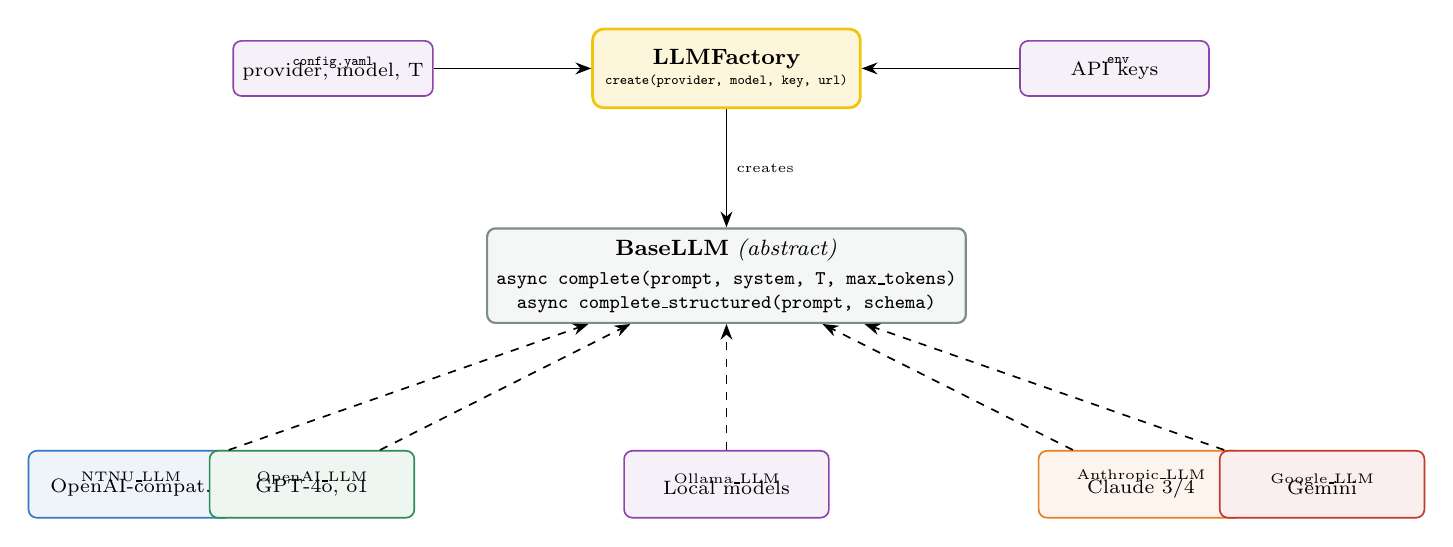
\begin{tikzpicture}[
    abstract/.style={rectangle, rounded corners=3pt, draw=agentgray, fill=agentgray!8, line width=0.8pt, minimum width=4.8cm, minimum height=1.2cm, align=center, font=\footnotesize},
    concrete/.style={rectangle, rounded corners=3pt, draw=#1, fill=#1!8, line width=0.6pt, minimum width=2.6cm, minimum height=0.85cm, align=center, font=\tiny},
    factory/.style={rectangle, rounded corners=4pt, draw=llmgold, fill=llmgold!15, line width=1pt, minimum width=3.4cm, minimum height=1.0cm, align=center, font=\footnotesize\bfseries},
    config/.style={rectangle, rounded corners=3pt, draw=agentpurple, fill=agentpurple!8, line width=0.6pt, minimum width=2.4cm, minimum height=0.7cm, align=center, font=\tiny},
    arr/.style={-{Stealth[length=2mm]}, semithick},
    darr/.style={-{Stealth[length=2mm]}, semithick, dashed}
]

% Abstract base
\node[abstract] (base) at (0,0) {\textbf{BaseLLM} \textit{(abstract)}\\[1pt]\texttt{\scriptsize async complete(prompt, system, T, max\_tokens)}\\[-1pt]\texttt{\scriptsize async complete\_structured(prompt, schema)}};

% Concrete implementations
\node[concrete=agentblue, below left=1.6cm and 3.2cm of base] (ntnu) {NTNU\_LLM\\[-2pt]\scriptsize OpenAI-compat.};
\node[concrete=agentgreen, below left=1.6cm and 0.9cm of base] (openai) {OpenAI\_LLM\\[-2pt]\scriptsize GPT-4o, o1};
\node[concrete=agentorange, below right=1.6cm and 0.9cm of base] (anthropic) {Anthropic\_LLM\\[-2pt]\scriptsize Claude 3/4};
\node[concrete=agentred, below right=1.6cm and 3.2cm of base] (google) {Google\_LLM\\[-2pt]\scriptsize Gemini};
\node[concrete=agentpurple, below=1.6cm of base] (ollama) {Ollama\_LLM\\[-2pt]\scriptsize Local models};

% Factory
\node[factory, above=1.5cm of base] (factory) {LLMFactory\\[-2pt]\tiny\texttt{create(provider, model, key, url)}};

% Config
\node[config, left=2.0cm of factory] (config) {\texttt{config.yaml}\\[-2pt]\scriptsize provider, model, T};
\node[config, right=2.0cm of factory] (env) {\texttt{.env}\\[-2pt]\scriptsize API keys};

% Inheritance arrows
\draw[darr] (ntnu) -- (base);
\draw[darr] (openai) -- (base);
\draw[darr] (ollama) -- (base);
\draw[darr] (anthropic) -- (base);
\draw[darr] (google) -- (base);

% Factory to base
\draw[arr] (factory) -- node[right, font=\tiny] {creates} (base);

% Config to factory
\draw[arr] (config) -- (factory);
\draw[arr] (env) -- (factory);

\end{tikzpicture}%
}% end resizebox
\caption{LLM provider abstraction architecture. The \texttt{LLMFactory} instantiates provider-specific implementations of the abstract \texttt{BaseLLM} interface based on runtime configuration. All providers expose identical asynchronous \texttt{complete()} and \texttt{complete\_structured()} methods.}
\label{fig:llm_architecture}
\end{figure}

The abstract \texttt{BaseLLM} class defines two core methods:
\begin{itemize}[leftmargin=*]
    \item \texttt{complete(prompt, system, temperature, max\_tokens)} $\to$ \texttt{str}: Free-form text generation for expert analysis and review.
    \item \texttt{complete\_structured(prompt, schema)} $\to$ Pydantic model: Structured output generation conforming to a specified JSON schema, used for extracting numerical recommendations (yaw angle, pitch angle, operating region).
\end{itemize}

Five concrete implementations are registered:
\begin{enumerate}[leftmargin=*]
    \item \textbf{NTNU HPC} (\texttt{ntnu\_llm.py}): Connects to the NTNU IDUN cluster via an OpenAI-compatible endpoint, supporting models such as Kimi-K2.5 and NorwAI-Magistral-24B. Implements retry logic with exponential backoff (3 attempts, 300\,s timeout).
    \item \textbf{OpenAI} (\texttt{openai\_llm.py}): Standard OpenAI API for GPT-4o, GPT-4o-mini, and o1-series models.
    \item \textbf{Anthropic} (\texttt{anthropic\_llm.py}): Anthropic API for Claude~3/4 models using the native \texttt{anthropic} client library.
    \item \textbf{Google} (\texttt{google\_llm.py}): Google Generative AI API for Gemini models.
    \item \textbf{Ollama} (\texttt{ollama.py}): Local model serving via the Ollama runtime, requiring no API key and supporting models such as LLaMA~3.2, Mistral, and Phi-3.
\end{enumerate}

\subsection{LLM as Turbine Expert (Agent~2B)}
\label{sec:llm_expert}

Agent~2B constructs a structured prompt containing:
\begin{itemize}[leftmargin=*]
    \item Current wind conditions (speed, direction, temperature) from Agent~1.
    \item NREL 5\,MW turbine specifications (126\,m rotor diameter, 90\,m hub height, 3--25\,m/s operating range).
    \item A request for optimal yaw angle, pitch angle, expected operating region, and reasoning.
\end{itemize}
The LLM's response is parsed via \texttt{complete\_structured()} into a typed data structure, enabling downstream agents to consume the recommendation programmatically.
By placing Agent~2B alongside the deterministic Agent~2A, operators can compare rule-based and AI-generated recommendations, building trust through cross-validation.

\subsection{LLM as Expert Reviewer}
\label{sec:llm_reviewer}

The expert reviewer (\texttt{reviewer\_agent.py}) operates at three checkpoints with a two-phase validation strategy:
\begin{enumerate}[leftmargin=*]
    \item \textbf{Rule-based checks}: Deterministic boundary validation (e.g., $270^\circ \leq \theta_{\text{yaw}} \leq 285^\circ$, $0 \leq P \leq 5$\,MW, $0 \leq v_\infty \leq 25$\,m/s) and consistency verification (operating region matches wind speed).
    \item \textbf{LLM-based reasoning}: The reviewer constructs a prompt containing the agent output, relevant context, and asks the LLM to assess physical plausibility, flag potential issues, and provide a confidence rating.
\end{enumerate}
The reviewer configuration (mode, temperature, provider) is specified in \texttt{config.yaml} and can optionally use the same or a different LLM provider from Agent~2B.


% ============================================================
% 5. WAKE STEERING OPTIMISATION
% ============================================================
\section{Wake Steering Optimisation}
\label{sec:optimisation}

\subsection{Single-Turbine Yaw Optimisation}

For a single upstream turbine, the optimal yaw angle is determined by maximising the GPR-predicted power while accounting for uncertainty:
\begin{equation}
    \theta_{\text{yaw}}^* = \arg\max_{\theta \in [\theta_{\min}, \theta_{\max}]} \; \mu_{\text{GP}}(\theta) - \kappa \cdot \sigma_{\text{GP}}(\theta)
\end{equation}
where $\mu_{\text{GP}}$ and $\sigma_{\text{GP}}$ are the GP posterior mean and standard deviation, and $\kappa \geq 0$ is a risk-aversion parameter (higher $\kappa$ favours yaw angles with lower uncertainty).

\subsection{Multi-Turbine Farm Optimisation}

For a farm of $N_T$ turbines, the optimiser integrates the GP power model with an analytical wake deficit model to maximise aggregate power:
\begin{equation}
    \max_{\boldsymbol{\theta}} \sum_{i=1}^{N_T} P_i(\boldsymbol{\theta}, v_\infty, \theta_w)
\end{equation}
where $\boldsymbol{\theta} = [\theta_1, \ldots, \theta_{N_T}]^T$ are the yaw angles and $P_i$ is the power of turbine~$i$ accounting for wake deficits from all upstream turbines.

The wake deficit at a downstream distance of $d/D$ rotor diameters is modelled as:
\begin{equation}
    \delta_u = \frac{1 - \sqrt{1 - C_T}}{(1 + 2k_w \cdot d/D)^2}
\end{equation}
where $C_T$ is the thrust coefficient and $k_w$ is the wake expansion coefficient.
Yaw-induced wake deflection shifts the wake centre laterally:
\begin{equation}
    \Delta y = \alpha_d \cdot \gamma \cdot d/D
\end{equation}
where $\gamma$ is the yaw misalignment and $\alpha_d$ is an empirical deflection coefficient.

\Cref{fig:optimisation} illustrates the optimisation loop.

% ============================================================
% FIGURE 4: Optimisation Loop
% ============================================================
\begin{figure}[H]
\centering
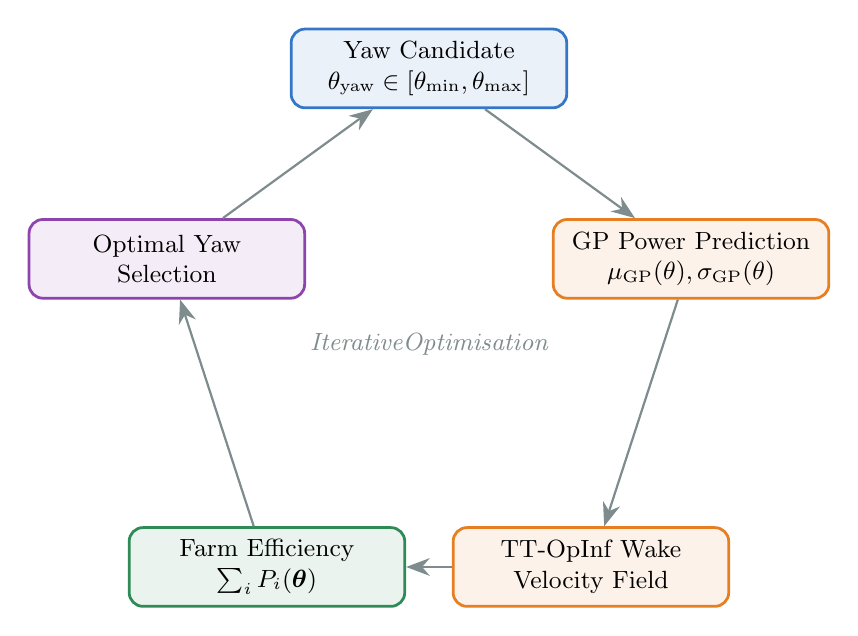
\begin{tikzpicture}[
    box/.style={rectangle, rounded corners=5pt, draw=#1, fill=#1!10, line width=1pt, minimum width=3.5cm, minimum height=1.0cm, align=center, font=\small},
    arr/.style={-{Stealth[length=3mm]}, thick, color=agentgray}
]

% Nodes in a circular layout
\node[box=agentblue] (cand) at (90:3.5cm) {Yaw Candidate\\$\theta_{\text{yaw}} \in [\theta_{\min}, \theta_{\max}]$};
\node[box=agentorange] (gp) at (18:3.5cm) {GP Power Prediction\\$\mu_{\text{GP}}(\theta), \sigma_{\text{GP}}(\theta)$};
\node[box=agentorange] (wake) at (-54:3.5cm) {TT-OpInf Wake\\Velocity Field};
\node[box=agentgreen] (farm) at (-126:3.5cm) {Farm Efficiency\\$\sum_i P_i(\boldsymbol{\theta})$};
\node[box=agentpurple] (opt) at (162:3.5cm) {Optimal Yaw\\Selection};

% Circular arrows
\draw[arr] (cand) -- (gp);
\draw[arr] (gp) -- (wake);
\draw[arr] (wake) -- (farm);
\draw[arr] (farm) -- (opt);
\draw[arr] (opt) -- (cand);

% Central label
\node[font=\small\itshape, color=agentgray] at (0,0) {Iterative\\Optimisation};

\end{tikzpicture}
\caption{Wake steering optimisation loop integrating GP power prediction and TT-OpInf wake field prediction for multi-turbine farm-level yaw optimisation.}
\label{fig:optimisation}
\end{figure}


% ============================================================
% 6. IMPLEMENTATION
% ============================================================
\section{Implementation}
\label{sec:implementation}

\subsection{Technology Stack}

The \textsc{AeroAgent} framework is implemented in Python~3.11+ and deployed as a Streamlit web application.
\Cref{tab:tech_stack} summarises the principal dependencies.

\begin{table}[H]
\centering
\caption{Technology stack and principal dependencies.}
\label{tab:tech_stack}
\small
\begin{tabular}{l l l}
\toprule
\textbf{Category} & \textbf{Library} & \textbf{Purpose} \\
\midrule
Web framework & Streamlit & Interactive GUI and deployment \\
Numerical computing & NumPy, SciPy & Array operations, SVD, RBF interpolation \\
Machine learning & scikit-learn 1.8 & GP, GMM, Random Forest, Gradient Boosting \\
Deep learning & PyTorch & Autoencoder training (PdM module) \\
Visualisation & Matplotlib, PyVista, Pydeck & 2D plots, 3D VTK rendering, map views \\
LLM clients & OpenAI, Anthropic, Google & API communication with LLM providers \\
Explainability & SHAP & Shapley-value-based model interpretation \\
Data handling & Pandas, joblib & Data manipulation, model serialisation \\
Configuration & PyYAML, python-dotenv & YAML config, environment variable management \\
\bottomrule
\end{tabular}
\end{table}

\subsection{GUI Architecture}

The Streamlit GUI (\texttt{wind\_turbine\_gui.py}) provides the following interactive pages:
\begin{enumerate}[leftmargin=*]
    \item \textbf{Overview}: System status, agent health, and quick-start guide.
    \item \textbf{Weather \& Wind Conditions}: Real-time weather data with geographic map integration for Norwegian wind farms (Bessaker, Sm{\o}la, Tonstad, Roan, Raggovidda).
    \item \textbf{Agent Analysis}: Individual agent outputs with expandable detail views.
    \item \textbf{Power Optimisation}: Single- and multi-turbine yaw optimisation with interactive sliders.
    \item \textbf{Wake Visualisation}: Animated three-dimensional velocity field rendering and VTK export.
    \item \textbf{Predictive Maintenance}: Health indicator time series, fault probability dashboards, RUL trends, and maintenance chatbot.
    \item \textbf{SHAP Analysis}: Interactive feature importance plots and per-sample explanations.
    \item \textbf{Settings}: LLM provider selection, model configuration, and API key management.
\end{enumerate}

The \texttt{GlobalLLMConfig} class manages persistent LLM configuration across Streamlit session state, enabling runtime switching between providers without page reloads.

\subsection{Norwegian Wind Farm Integration}

The framework includes geocoded locations and specifications for five Norwegian wind farms:
\begin{itemize}[leftmargin=*]
    \item \textbf{Bessaker} (25 turbines, 57.5\,MW) --- {\AA}fjord, Tr{\o}ndelag
    \item \textbf{Sm{\o}la} (68 turbines, 150\,MW) --- one of Norway's oldest large farms
    \item \textbf{Tonstad} (51 turbines, 208\,MW) --- one of Norway's largest onshore farms
    \item \textbf{Roan} (71 turbines, 255.6\,MW) --- part of the Fosen Vind project
    \item \textbf{Raggovidda} (15 turbines, 45\,MW) --- Norway's northernmost farm
\end{itemize}
For each farm, turbine positions are used for map rendering and inter-turbine distance calculations in the wake steering optimiser.


% ============================================================
% 7. RESULTS AND DISCUSSION
% ============================================================
\section{Results and Discussion}
\label{sec:results}

This section presents representative outputs from the integrated multi-agent framework and discusses the advantages of the agentic approach.

\subsection{Wake Flow Prediction}

\Cref{fig:wake_analysis} shows the wake deficit as a function of inter-turbine spacing for varying upstream yaw angles, computed by integrating the TT-OpInf velocity field predictions with the analytical wake deficit model.
The results demonstrate that yaw misalignment reduces the wake deficit experienced by downstream turbines at the cost of reduced upstream power, confirming the fundamental trade-off in wake steering optimisation.

\begin{figure}[H]
    \centering
    \includegraphics[width=0.85\textwidth]{wake_deficit_spacing_analysis.png}
    \caption{Wake deficit as a function of downstream spacing (in rotor diameters) for varying upstream yaw angles. Increased yaw misalignment deflects the wake laterally, reducing the deficit at typical inter-turbine spacings of 5--7$D$.}
    \label{fig:wake_analysis}
\end{figure}

\subsection{Rotor Power Prediction}

\Cref{fig:power_prediction} presents the GPR power predictions across yaw angles, showing the mean power trajectory with 95\% confidence intervals.
The GP model captures the transient power dynamics during yaw angle changes while providing calibrated uncertainty bounds that widen at extrapolated conditions.

\begin{figure}[H]
    \centering
    \includegraphics[width=0.85\textwidth]{rotor_power_variation_by_yaw.png}
    \caption{Rotor power variation by yaw angle. The GP model predicts both mean power and uncertainty (shaded region), enabling risk-aware decision-making in the optimisation loop.}
    \label{fig:power_prediction}
\end{figure}

\begin{figure}[H]
    \centering
    \includegraphics[width=0.85\textwidth]{model_evaluation.png}
    \caption{GP model evaluation: predicted vs.\ actual power, residual distribution, and confidence interval calibration on the held-out test set (RMSE~$= 0.048$\,MW, $R^2 = 0.70$).}
    \label{fig:model_eval}
\end{figure}

\subsection{Predictive Maintenance}

\Cref{fig:pdm_analysis} presents the four-stage PdM pipeline results on the Fuhrlander FL2500 dataset, including autoencoder convergence, Health Indicator distribution by GMM state, feature importance, and RUL predictions.
The Health Indicator exhibits clear separation between healthy and degraded states, with the GMM identifying three distinct operational regimes.

\begin{figure}[H]
    \centering
    \includegraphics[width=0.95\textwidth]{fuhrlander_pm_analysis.png}
    \caption{Predictive maintenance pipeline results. Row~1: Dataset overview. Row~2: Autoencoder convergence (left) and Health Indicator with GMM states (right). Row~3: Test turbine HI time series. Row~4: Feature importance. Row~5: RUL predictions at fault events.}
    \label{fig:pdm_analysis}
\end{figure}

\Cref{fig:inference_dashboard} shows the real-time inference dashboard for turbine~83, demonstrating the integrated health assessment with multi-model consensus.

\begin{figure}[H]
    \centering
    \includegraphics[width=0.85\textwidth]{inference_turbine_83_dashboard.png}
    \caption{Real-time health assessment dashboard for turbine~83, showing Health Indicator trend, GMM state classification, fault probability, and RUL estimate.}
    \label{fig:inference_dashboard}
\end{figure}

\subsection{SHAP Explainability}

\Cref{fig:shap_dashboard} presents the SHAP analysis dashboard, showing global feature importance and per-sample explanations.
The analysis confirms that oil pressure features (bearing and gearbox) are the strongest predictors of fault conditions, consistent with known gearbox degradation physics where lubrication system degradation precedes bearing surface damage \citep{igba2015}.

\begin{figure}[H]
    \centering
    \includegraphics[width=0.85\textwidth]{shap_dashboard.png}
    \caption{SHAP explainability dashboard. Top: Global feature importance comparison (SHAP vs.\ Mean Decrease in Impurity). Bottom: Beeswarm plot showing feature impact distribution across samples.}
    \label{fig:shap_dashboard}
\end{figure}

\subsection{Discussion}

\subsubsection{Benefits of the Multi-Agent Architecture}

The agentic framework provides several advantages over monolithic approaches:
\begin{itemize}[leftmargin=*]
    \item \textbf{Modularity}: Each agent can be developed, tested, and updated independently. The TT-OpInf model can be retrained on new CFD data without affecting the PdM pipeline, and LLM providers can be switched at runtime.
    \item \textbf{Cross-validation}: The dual expert system (rule-based Agent~2A and LLM-based Agent~2B) enables operators to compare deterministic and AI-generated recommendations, building trust through consensus.
    \item \textbf{Quality assurance}: The checkpoint-based reviewer system provides systematic validation, catching physically implausible predictions before they propagate downstream.
    \item \textbf{Extensibility}: New agents (e.g., structural health monitoring, grid integration analysis) can be added to the orchestrator without modifying existing agents.
\end{itemize}

\subsubsection{LLM Integration Considerations}

The multi-provider abstraction enables deployment flexibility: organisations with HPC access can use locally hosted models via NTNU or Ollama for data privacy, while cloud-based providers (OpenAI, Anthropic, Google) offer state-of-the-art reasoning capabilities.
The LLM reviewer adds value beyond simple rule-based checks by providing contextual reasoning about result plausibility, particularly for edge cases that are difficult to encode deterministically (e.g., simultaneous high wind speed and low power output that could indicate either curtailment or fault).

\subsubsection{Uncertainty Quantification}

The GPR model's built-in uncertainty quantification is a distinctive advantage over point-estimate surrogates.
The 95\% confidence intervals propagate through the optimisation loop, enabling risk-aware yaw control where the operator can balance expected power gain against prediction uncertainty.
This probabilistic framework is particularly valuable during transient conditions or at operating points far from the training data, where model extrapolation is inherently uncertain.

\subsubsection{Scalability}

The current framework supports single-turbine and small farm analyses.
Scaling to large farms (50+ turbines) would require:
\begin{itemize}[leftmargin=*]
    \item Parallel execution of agents using asynchronous task queues.
    \item Sparse GP approximations \citep{Titsias2009} or scalable GP implementations for the power surrogate.
    \item Additional training data for the TT-OpInf model covering a wider range of yaw angles and atmospheric conditions.
\end{itemize}


% ============================================================
% 8. CONCLUSION
% ============================================================
\section{Conclusion}
\label{sec:conclusion}

This report has presented \textsc{AeroAgent}, a multi-agent AI framework that integrates Large Language Models with domain-specific machine learning surrogates for wind turbine operational analysis.
The framework comprises six specialised agents orchestrated through a checkpoint-based pipeline with LLM-powered expert review.

The constituent ML models demonstrate competitive performance on their respective tasks:
\begin{itemize}[leftmargin=*]
    \item The TT-OpInf ROM achieves $10.1\times$ data compression with 12.9\% relative $L^2$ error for wake field prediction, enabling sub-second inference on 180{,}857 spatial nodes without GPU requirements.
    \item The GPR power surrogate provides uncertainty-aware predictions with RMSE of 0.048\,MW and $R^2 = 0.70$, enabling risk-aware yaw optimisation.
    \item The semi-supervised PdM pipeline achieves a weighted F1-score of 0.75 on real SCADA data, with 76.3\% of fault events detected within a 50-hour window.
\end{itemize}

The multi-provider LLM abstraction layer supports five providers through a unified interface, enabling deployment flexibility from local models to cloud-based state-of-the-art systems.
SHAP-based explainability at each prediction stage ensures model transparency and builds operator trust.

\subsection{Future Work}

Several directions are identified for future development:
\begin{enumerate}[leftmargin=*]
    \item \textbf{Real-time deployment}: Integration with turbine SCADA systems for online monitoring and closed-loop yaw control.
    \item \textbf{Domain-specific LLM fine-tuning}: Training specialised language models on wind energy technical literature, operational logs, and maintenance records to improve the quality of expert recommendations.
    \item \textbf{Digital twin integration}: Coupling the framework with a physics-based digital twin for hybrid model--data assimilation and model validation.
    \item \textbf{Reinforcement learning}: Replacing the static optimisation loop with an RL agent that learns yaw control policies through interaction with the TT-OpInf and GP surrogates.
    \item \textbf{Fleet-level analytics}: Extending the PdM module to exploit cross-turbine correlations for fleet-level health monitoring and maintenance scheduling.
    \item \textbf{Retrieval-Augmented Generation (RAG)}: Augmenting the LLM expert with a vector database of turbine manuals, maintenance records, and incident reports for context-aware recommendations.
\end{enumerate}


% ============================================================
% REFERENCES
% ============================================================
\bibliographystyle{plainnat}
\bibliography{technical_report_multiagent}

\end{document}
